\chapter{Data model}\label{Chap:DataModel}
\begin{figure}[!htb]
   \centering
   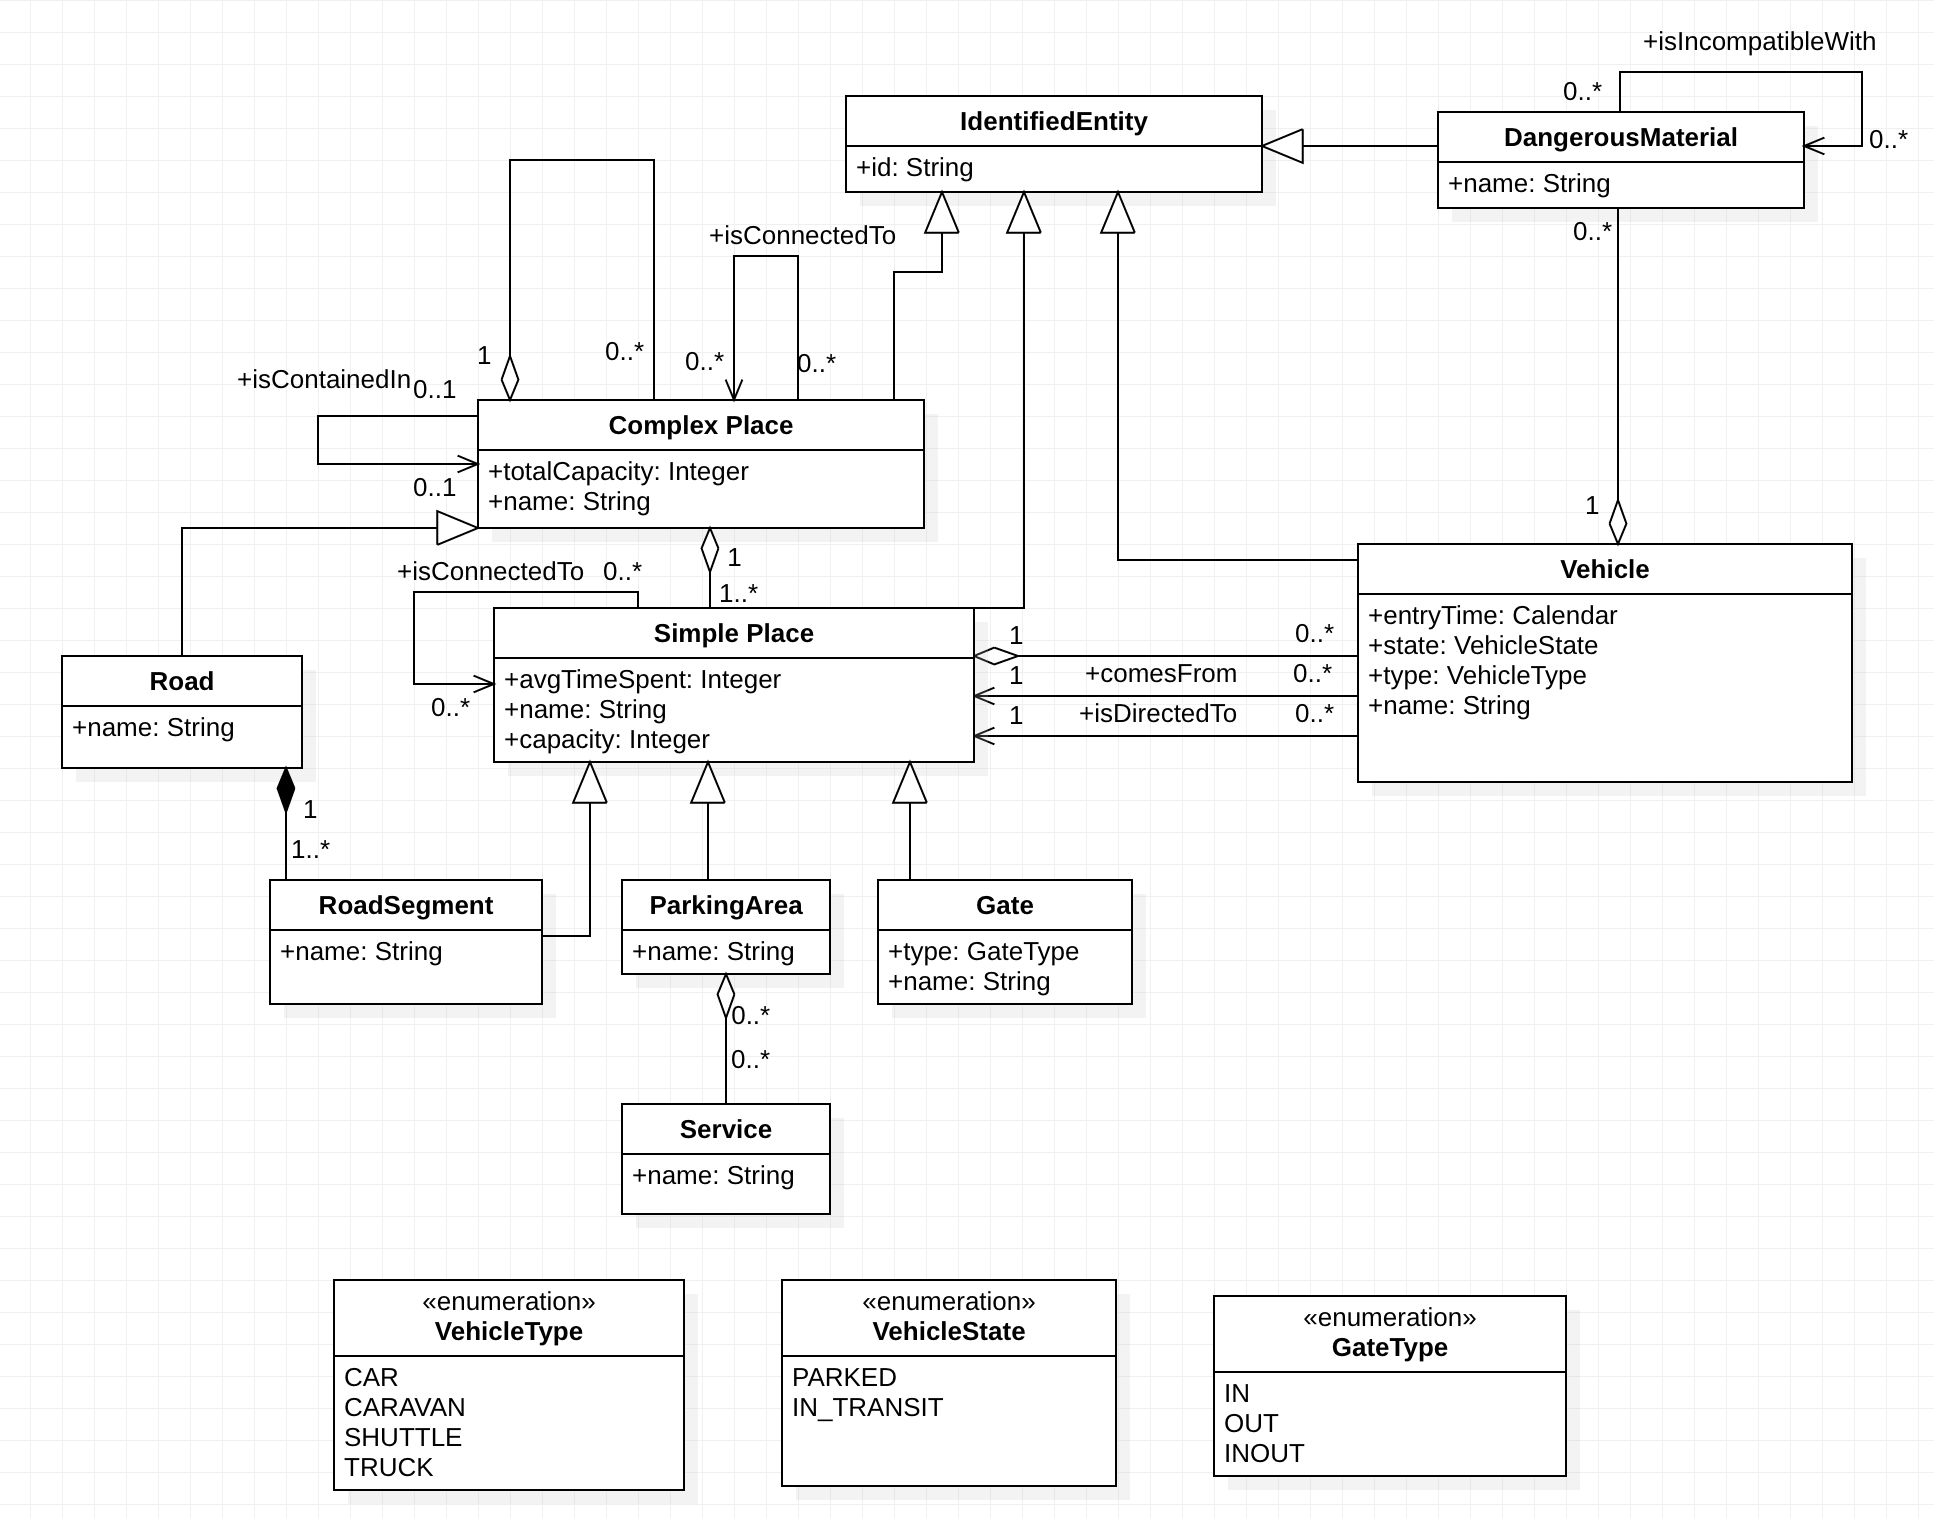
\includegraphics[width=\textwidth]{data_model.png}
   \caption{Data model for the application.}\label{Fig:ArchNoImpl}
\end{figure}
In figure \ref{Fig:ArchNoImpl} it is represented the UML model it has been referred to in order to describe the data the application will handle. Each node of the map can be described as a simple place and each place has a maximum capacity, that represents the maximum number of vehicle that can be at the same time in that place. This property of the places will be exploited as constraint during the evaluation of a path for the entering vehicles. Particularity of this model is the presence of complex places that are a particular type of place. They have been defined in such way that they can contain a set of simple places or other complex places. For this particular project has been defined only one type of complex place: Road. Such type of place is a collection of RoadSegments. If for future use purposes it is necessary to add other particular complex places, it is necessary to extends the ComplexPlace type, as in the case of Road.\\
All the information regarding the schema representing the model and from which the Java classes have been generated with JAXB, are contained in file \textit{RnsInfo.xsd}.
